\documentclass[12pt, a4paper, oneside, openright, titlepage]{book}
\usepackage[utf8]{inputenc}
\raggedbottom
\usepackage{import}


%%%%%%%%%%%%%%%%% Book Formatting Comments:

%%%%%%%%%%%%%%%%%%%%%%%%%%%%%%%%%%%%% for Part

%%%%%%%%%%%%%%%%%%%%%% for chapter

%%%%%%%%%%%%%%%%%%%% for section








%%%%%% PACKAGES %%%%%%%
\usepackage{hyperref}
\hypersetup{
    colorlinks,
    citecolor=black,
    filecolor=black,
    linkcolor=black,
    urlcolor=black
}
\usepackage{amsmath} % Math display options
\usepackage{amssymb} % Math symbols
\usepackage{amsfonts} % Math fonts
\usepackage{amsthm}
\usepackage{mathtools} % General math tools
\usepackage{array} % Allows you to write arrays
\usepackage{empheq} % For boxing equations
\usepackage{mathabx}
\usepackage{mathrsfs}
\usepackage{nameref}

\usepackage{soul}
\usepackage[normalem]{ulem}

\usepackage{txfonts}
\usepackage{cancel}
\usepackage[toc, page]{appendix}
\usepackage{titletoc,tocloft}
\setlength{\cftchapindent}{1em}
\setlength{\cftsecindent}{2em}
\setlength{\cftsubsecindent}{3em}
\setlength{\cftsubsubsecindent}{4em}
\usepackage{titlesec}

\titleformat{\section}
  {\normalfont\fontsize{25}{15}\bfseries}{\thesection}{1em}{}
\titleformat{\section}
  {\normalfont\fontsize{20}{15}\bfseries}{\thesubsection}{1em}{}
\setcounter{secnumdepth}{1}  
  
  

\newcommand\numberthis{\refstepcounter{equation}\tag{\theequation}} % For equation labelling
\usepackage[framemethod=tikz]{mdframed}

\usepackage{tikz} % For drawing commutative diagrams
\usetikzlibrary{cd}
\usetikzlibrary{calc}
\tikzset{every picture/.style={line width=0.75pt}} %set default line width to 0.75p

\usepackage{datetime}
\usepackage[margin=1in]{geometry}
\setlength{\parskip}{1em}
\usepackage{graphicx}
\usepackage{float}
\usepackage{fancyhdr}
\setlength{\headheight}{15pt} 
\pagestyle{fancy}
\lhead[\leftmark]{}
\rhead[]{\leftmark}

\usepackage{enumitem}

\usepackage{url}
\allowdisplaybreaks

%%%%%% ENVIRONMENTS %%%
\definecolor{purp}{rgb}{0.29, 0, 0.51}
\definecolor{bloo}{rgb}{0, 0.13, 0.80}



%%\newtheoremstyle{note}% hnamei
%{3pt}% hSpace above
%{3pt}% hSpace belowi
%{}% hBody fonti
%{}% hIndent amounti
%{\itshape}% hTheorem head fonti
%{:}% hPunctuation after theorem headi
%{.5em}% hSpace after theorem headi
%{}% hTheorem head spec (can be left empty, meaning ‘normal’)i


%%%%%%%%%%%%% THEOREM STYLES

\newtheoremstyle{BigTheorem}
{20pt}
{20pt}
{\slshape}
{}
{\Large\color{purp}\bfseries}
{.}
{\newline}
{\thmname{#1}\thmnumber{ #2}\thmnote{ (#3)}}



\newtheoremstyle{TheoremClassic}
{15pt}
{15pt}
{\slshape}
{}
{\bfseries}
{.}
{.5em}
{}

\newtheoremstyle{Definitions}
{15pt}
{15pt}
{\slshape}
{}
{\bfseries}
{.}
{.5em}
{\thmname{#1}\thmnumber{ #2}\thmnote{ (#3)}}


\newtheoremstyle{Remarks}
{10pt}
{10pt}
{\upshape}
{}
{\bfseries}
{.}
{.5em}
{}

\newtheoremstyle{Examples}
{10pt}
{10pt}
{\upshape}
{}
{\bfseries}
{.}
{.5em}
{}


%%%%%%%%%%%%% THEOREM DEFINITIONS

\theoremstyle{BigTheorem}
\newtheorem{namthm}{Theorem}
\newtheorem{conj}[namthm]{Conjecture}

\theoremstyle{TheoremClassic}
\newtheorem{thm}{Theorem}[section]
\newtheorem*{thm*}{Theorem}
\newtheorem{lem}[thm]{Lemma}
\newtheorem{cor}[thm]{Corollary}
\newtheorem{prop}[thm]{Proposition}
\newtheorem{claim}[thm]{Claim}


\theoremstyle{Definitions}
\newtheorem{defn}{Definition}[section]
\newtheorem{axi}[defn]{Axiom}
\newtheorem{cust}[defn]{}
\newtheorem{cons}[defn]{Construction}
\newtheorem{props}[defn]{Properties}
\newtheorem{proc}[defn]{Process}
\newtheorem*{law}{Law}


\theoremstyle{Examples}
\newtheorem{eg}{Example}[section]
\newtheorem{noneg}[eg]{Non-Example}
\newtheorem{xca}[eg]{Exercise}


\theoremstyle{Remarks}
\newtheorem{rmk}{Remark}[section]
\newtheorem{qst}[rmk]{Question}
\newtheorem*{ans}{Answer}
\newtheorem{obs}[rmk]{Observation}
\newtheorem{rec}[rmk]{Recall}
\newtheorem{summ}[rmk]{Summary}
\newtheorem{nota}[rmk]{Notation}
\newtheorem{note}[rmk]{Note}



\renewcommand{\qedsymbol}{$\blacksquare$}


\numberwithin{equation}{section}

\newenvironment{qest}{
    \begin{center}
        \em
    }
    {
    \end{center}
    }

%%%%%% MACROS %%%%%%%%%
%% New Commands
\newcommand{\ip}[1]{\langle#1\rangle} %%% Inner product
\newcommand{\abs}[1]{\lvert#1\rvert} %%% Modulus
\newcommand\diag{\operatorname{diag}} %%% diag matrix
\newcommand\tr{\mbox{tr}\.} %%% trace
\newcommand\C{\mathbb C} %%% Complex numbers
\newcommand\R{\mathbb R} %%% Real numbers
\newcommand\Z{\mathbb Z} %%% Integers
\newcommand\Q{\mathbb Q} %%% Rationals
\newcommand\N{\mathbb N} %%% Naturals
\newcommand\F{\mathbb F} %%% An arbitrary field
\newcommand\ste{\operatorname{St}} %%% Steinberg Representation
\newcommand\GL{\mathbf{GL}} %%% General Linear group
\newcommand\SL{\mathbf{SL}} %%% Special linear group
\newcommand\gl{\mathfrak{gl}} %%% General linear algebra
\newcommand\G{\mathbf{G}} %%% connected reductive group
\newcommand\g{\mathfrak{g}} %%% Lie algebra of G
\newcommand\Hbf{\mathbf{H}} %%% Theta fixed points of G
\newcommand\X{\mathbf{X}} %%% Symmetric space X
\newcommand{\catname}[1]{\normalfont\textbf{#1}}
\newcommand{\Set}{\catname{Set}} %%% Category set
\newcommand{\Grp}{\catname{Grp}} %%% Category group
\newcommand{\Rmod}{\catname{R-Mod}} %%% Category r-modules
\newcommand{\Mon}{\catname{Mon}} %%% Category monoid
\newcommand{\Ring}{\catname{Ring}} %%% Category ring
\newcommand{\Topp}{\catname{Top}} %%% Category Topological spaces
\newcommand{\Vect}{\catname{Vect}_{k}} %%% category vector spaces'
\newcommand\Hom{\mathbf{Hom}} %%% Arrows

\newcommand{\map}[2]{\begin{array}{c} #1 \\ #2 \end{array}}

\newcommand{\Emph}[1]{\textbf{\ul{\emph{#1}}}}

\newcommand{\mapsfrom}{\mathrel{\reflectbox{\ensuremath{\mapsto}}}}


%% Math operators
\DeclareMathOperator{\ran}{Im} %%% image
\DeclareMathOperator{\aut}{Aut} %%% Automorphisms
\DeclareMathOperator{\spn}{span} %%% span
\DeclareMathOperator{\ann}{Ann} %%% annihilator
\DeclareMathOperator{\rank}{rank} %%% Rank
\DeclareMathOperator{\ch}{char} %%% characteristic
\DeclareMathOperator{\ev}{\bf{ev}} %%% evaluation
\DeclareMathOperator{\sgn}{sign} %%% sign
\DeclareMathOperator{\id}{Id} %%% identity
\DeclareMathOperator{\supp}{Supp} %%% support
\DeclareMathOperator{\inn}{Inn} %%% Inner aut
\DeclareMathOperator{\en}{End} %%% Endomorphisms
\DeclareMathOperator{\sym}{Sym} %%% Group of symmetries


%% Diagram Environments
\iffalse
\begin{center}
    \begin{tikzpicture}[baseline= (a).base]
        \node[scale=1] (a) at (0,0){
          \begin{tikzcd}
           
          \end{tikzcd}
        };
    \end{tikzpicture}
\end{center}
\fi




\newdateformat{monthdayyeardate}{%
    \monthname[\THEMONTH]~\THEDAY, \THEYEAR}
%%%%%%%%%%%%%%%%%%%%%%%

%%% Specific Macros %%%


%%%%%% BEGIN %%%%%%%%%%


\begin{document}

%%%%%% TITLE PAGE %%%%%

\begin{titlepage}
    \centering
    \scshape
    \vspace*{\baselineskip}
    \rule{\textwidth}{1.6pt}\vspace*{-\baselineskip}\vspace*{2pt}
    \rule{\textwidth}{0.4pt}
    
    \vspace{0.75\baselineskip}
    
    {\LARGE Statistical Mechanics: A Complete Guide}
    
    \vspace{0.75\baselineskip}
    
    \rule{\textwidth}{0.4pt}\vspace*{-\baselineskip}\vspace{3.2pt}
    \rule{\textwidth}{1.6pt}
    
    \vspace{2\baselineskip}
    Phys 449 \\
    \vspace*{3\baselineskip}
    \monthdayyeardate\today \\
    \vspace*{5.0\baselineskip}
    
    {\scshape\Large Elijah Thompson, \\ Physics and Math Honors\\}
    
    \vspace{1.0\baselineskip}
    \textit{Solo Pursuit of Learning}
    \vfill
    \enlargethispage{1in}
    \begin{figure}[b!]
    \makebox[\textwidth]{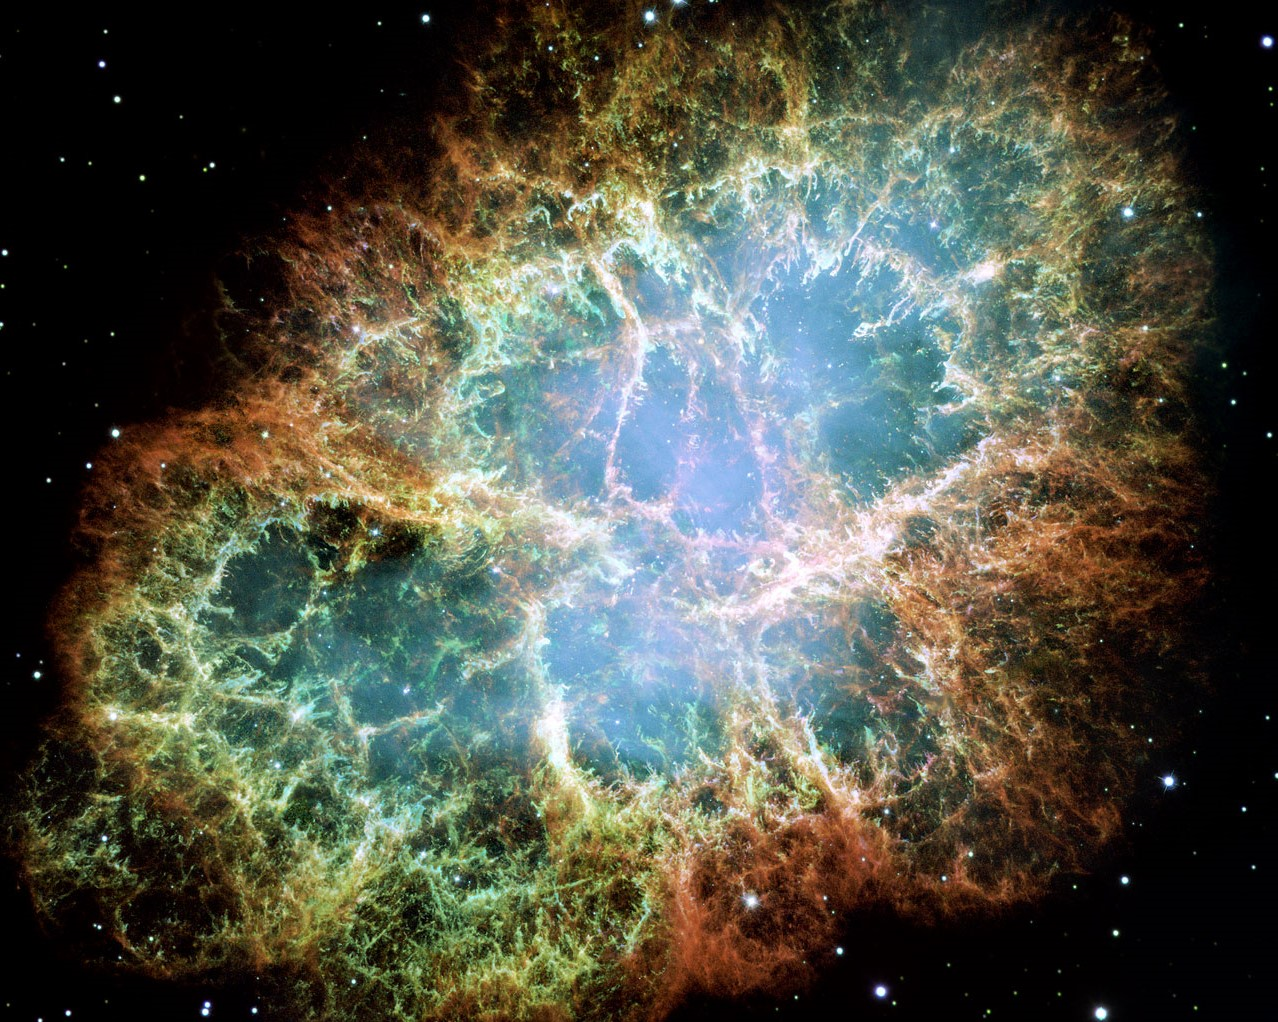
\includegraphics[width=\paperwidth, height =10cm]{../Crab.jpg}}
    \end{figure}
\end{titlepage}

%%%%%%%%%%%%%%%%%%%%%%%
\tableofcontents



%%%%%%%%%%%%%%%%%%%%%%%%%%%%%%%%%%%%% Part 1
\part{Thermodynamics}

%%%%%%%%%%%%%%%%%%%%%% Chapter 1.1
\chapter{Energy in Thermal Physics}

%%%%%%%%%%%%%%%%%%%% Section 1.1.1
\section{Basic Notation and Work}

\begin{defn}
    Thermodynamics is a \Emph{phenomenological} description of properties of \Emph{macroscopic systems} in \Emph{thermal equilibrium}.
\end{defn}

By a phenomenological description we mean a discription based on observations and direct experience of the experimenter with the system, considered as a ``black box" (a system whose internal structure is unknown, or is just not considered).

\begin{defn}[Systems]
    There are a number of different thermodynamic systems. We summarize them as follows: \begin{itemize}
        \item \Emph{Thermodynamic or Macroscopic System:} A system consisting of a large number of constituents. For example, a mole of gas (approximately $10^{23}$ particles) can be considered as a macroscopic system.
        \item \Emph{Isolated Thermodynamic System:} A system which exhibits no exchange of any type with the surroundings; no exchange of work, heat, matter, etc.
        \item \Emph{Closed Theormodynamic System:} A system which exhibits no exchange of matter with its surroundings.
        \item \Emph{Open Thermodynamic System:} A system for which it is possible for exchange of any type with the surroundings (work, heat, matter, etc.)
    \end{itemize}
\end{defn}

\begin{defn}[Equilibrium]
    Two thermodynamic systems are in \Emph{equilibrium} if and only if they are in contact such that they can exchange a given conserved quantity (for example particles) and they are relaxed to a state in which there is no average net transfer of that quantity between them anymore. A thermodynamic system $S$ is in equilibrium with itself, if and only if, all its subsystems are in equilibrium with each other. In this case, $S$ is called an \Emph{equilibrium} system.
\end{defn}

From this definition we find that different types of exchanged quanitities can lead to different types of equilibria: 

\begin{table}[H]
    \centering
    \begin{tabular}{c|c}
        \hline
        Exchanged Quantity & Type of Equilibrium \\ \hline \hline
        Particles/Matter & Diffusive Equilibrium \\ 
        Work & Mechanical Equilibrium \\
        Heat & Thermal Equilibrium \\ \hline
    \end{tabular}
\end{table}

\begin{defn}
    \Emph{Complete Thermodynamic Equilibrium} corresponds to a state where all the conserved fluxes between two coupled thermodynamic systems vanish.
\end{defn}

A way of testing if a given system is in a complete thermodynamic equilibrium is if the properties of the system do not change appreciably over the observation time, which is to say the properties reflect the true asymptotic long-term properties after any initial relaxation time is over.

The state of thermodynamic systems in complete thermodynamic equilibrium can be described by a set of independent \Emph{thermodynamic coordinates} or \Emph{state variables}; this fact is based on empirical observations. 

\subsection{Boyle-Mariotte's Experiment}

\begin{law}
    For a given mass of gas at a constant temperature $T$, the volume $V$ is inverseley proportional to the pressure $P$: $V \propto P^{-1}$.
\end{law}

We consider Robert Boyle's (1627-1691) experiment, conducted at room temperature, which should remain constant during the time of the experiment. We use a vertical tube with markings to indicate the volume of gas, and oil at the bottom. By applying pressure on the oil, we also exert a pressure on the air in the tube above the oil, causing the volume to decrease. Drawing the graph of volume versus $P^{-1}$ we obtain a straight line, so $V\cdot P = C$ for some constant $C$, given a fixed temperature. As further measurements show, the constant is proportional to the temperature $T$, so $V\cdot P \propto T$. More precisely, the full equation of a state of simple low-density gase is given by \begin{equation}
    \boxed{PV = Nk_BT}
\end{equation}
where $N$ is the number of gas particles and $k_B \approx 1.381\times 10^{-23}\;J/K$ is a natural constant called the \Emph{Boltzmann's constant}. The above equation is called the \Emph{ideal gas law} or the \Emph{equation of state for an ideal gas} since it relates the three state variables, or thermodynamic coordinates, $P$, $V$, and $T$ at equilibrium.





\subsection{Work}

\begin{defn}
    Given a vector force field $\vec{F}$ defined along a path $\gamma$, the \Emph{work} $W$ is of $\vec{F}$ along $\gamma$ is defined to be: \begin{equation}
        W = \int_{\gamma}\vec{F}\cdot d\vec{r}
    \end{equation}
\end{defn}

\begin{rec}
    Recall that pressure is force per unit area, so we have that \begin{equation*}
        P = \frac{F}{A}
    \end{equation*}
    where $F$ is the normal component of the force to the area $A$. More precisely, pressure is the proportionality constant that relates the force and normal vectors: \begin{equation*}
        d\vec{F}_n = -pd\vec{A}
    \end{equation*}
    where $\vec{F}_n$ denotes the normal component of the force vector $\vec{F}$.
\end{rec}


\begin{eg}
    Consider the compression of a gas by a piston with a constant force of magnitude $F$.
    \begin{center}
    \begin{tikzpicture}[x=0.75pt,y=0.75pt,yscale=-1.2,xscale=1.2]
%uncomment if require: \path (0,398); %set diagram left start at 0, and has height of 398

%Shape: Rectangle [id:dp9125760638904235] 
\draw   (100,110) -- (200,110) -- (200,160) -- (100,160) -- cycle ;
%Straight Lines [id:da19743423815417427] 
\draw    (200,110) -- (230,110) ;
%Straight Lines [id:da17599416360044806] 
\draw    (200,160) -- (230,160) ;
%Straight Lines [id:da37025754978607806] 
\draw [color={rgb, 255:red, 255; green, 27; blue, 0 }  ,draw opacity=1 ]   (200,110) -- (200,160) ;
%Straight Lines [id:da5752016333947421] 
\draw [color={rgb, 255:red, 255; green, 27; blue, 0 }  ,draw opacity=1 ]   (200,135) -- (250,135) ;
%Straight Lines [id:da4588247522685671] 
\draw    (230,127) -- (222,127) ;
\draw [shift={(220,127)}, rotate = 360] [color={rgb, 255:red, 0; green, 0; blue, 0 }  ][line width=0.75]    (4.37,-1.32) .. controls (2.78,-0.56) and (1.32,-0.12) .. (0,0) .. controls (1.32,0.12) and (2.78,0.56) .. (4.37,1.32)   ;
%Curve Lines [id:da22459360243367987] 
\draw [line width=0.75]    (281.89,123.39) .. controls (280.27,107.22) and (224.4,110.81) .. (204.92,121.69) ;
\draw [shift={(203.22,122.72)}, rotate = 326.56] [color={rgb, 255:red, 0; green, 0; blue, 0 }  ][line width=0.75]    (6.56,-1.97) .. controls (4.17,-0.84) and (1.99,-0.18) .. (0,0) .. controls (1.99,0.18) and (4.17,0.84) .. (6.56,1.97)   ;
%Straight Lines [id:da04861500853364609] 
\draw    (200,170) -- (192,170) ;
\draw [shift={(190,170)}, rotate = 360] [color={rgb, 255:red, 0; green, 0; blue, 0 }  ][line width=0.75]    (4.37,-1.32) .. controls (2.78,-0.56) and (1.32,-0.12) .. (0,0) .. controls (1.32,0.12) and (2.78,0.56) .. (4.37,1.32)   ;
%Straight Lines [id:da2692578781738837] 
\draw    (200,167) -- (200,173) ;

% Text Node
\draw (231,122.4) node [anchor=north west][inner sep=0.75pt]  [font=\tiny,color={rgb, 255:red, 246; green, 12; blue, 12 }  ,opacity=1 ]  {$\vec{F}$};
% Text Node
\draw (237,125) node [anchor=north west][inner sep=0.75pt]  [font=\tiny] [align=left] {(const.)};
% Text Node
\draw (270.89,125.89) node [anchor=north west][inner sep=0.75pt]  [font=\tiny] [align=left] {Piston area:};
% Text Node
\draw (311.89,125.4) node [anchor=north west][inner sep=0.75pt]  [font=\tiny,color={rgb, 255:red, 255; green, 0; blue, 0 }  ,opacity=1 ]  {$\mathcal{A}$};
% Text Node
\draw (108.56,114.4) node [anchor=north west][inner sep=0.75pt]  [font=\small]  {$\cdot $};
% Text Node
\draw (128.56,134.4) node [anchor=north west][inner sep=0.75pt]  [font=\small]  {$\cdot $};
% Text Node
\draw (128.56,134.4) node [anchor=north west][inner sep=0.75pt]  [font=\small]  {$\cdot $};
% Text Node
\draw (139.89,121.07) node [anchor=north west][inner sep=0.75pt]  [font=\small]  {$\cdot $};
% Text Node
\draw (159.89,141.07) node [anchor=north west][inner sep=0.75pt]  [font=\small]  {$\cdot $};
% Text Node
\draw (127.56,112.07) node [anchor=north west][inner sep=0.75pt]  [font=\small]  {$\cdot $};
% Text Node
\draw (161.56,117.4) node [anchor=north west][inner sep=0.75pt]  [font=\small]  {$\cdot $};
% Text Node
\draw (181.56,137.4) node [anchor=north west][inner sep=0.75pt]  [font=\small]  {$\cdot $};
% Text Node
\draw (110.22,132.4) node [anchor=north west][inner sep=0.75pt]  [font=\small]  {$\cdot $};
% Text Node
\draw (179.22,114.73) node [anchor=north west][inner sep=0.75pt]  [font=\small]  {$\cdot $};
% Text Node
\draw (142.89,141.4) node [anchor=north west][inner sep=0.75pt]  [font=\small]  {$\cdot $};
% Text Node
\draw (168.22,127.73) node [anchor=north west][inner sep=0.75pt]  [font=\small]  {$\cdot $};
% Text Node
\draw (148.22,112.73) node [anchor=north west][inner sep=0.75pt]  [font=\small]  {$\cdot $};
% Text Node
\draw (123.56,124.07) node [anchor=north west][inner sep=0.75pt]  [font=\small]  {$\cdot $};
% Text Node
\draw (111.56,142.73) node [anchor=north west][inner sep=0.75pt]  [font=\small]  {$\cdot $};
% Text Node
\draw (192,173.4) node [anchor=north west][inner sep=0.75pt]  [font=\tiny]  {$\Delta x$};


\end{tikzpicture}
\end{center}
    so the work is \begin{equation*}
        W = \int_{\gamma}\vec{F}\cdot d\vec{r} = F\int_{\gamma}dr = F\Delta x = PA\Delta x = -P\Delta V
    \end{equation*}
    where $P$ is the pressure and $\Delta V$ is the change in volume. Since the change in volume is negative, the work $W$ done on the system (here the gas) is positive: Energy is added to the system by a force (macroscopic) process (here the piston). $W< 0$ if energy is removed from the system.
\end{eg}


\begin{defn}
    The generalized differential form for work is given by \begin{equation}
        \delta W = \sum_{i=1}^mJ_idq_i
    \end{equation}
    where $q_i$ are the generalized coordinates and the $J_i$ are the conjugate generalized forces such that $J_idq_i$ has units of energy.
\end{defn}

Here are a few examples of generalized coordinates and their corresponding generalized conjugate forces:

\begin{table}[H]
    \centering
    \begin{tabular}{c|c|c}
        \hline
        & Generalized Force $J_i$ & Generalized Coordinate $dq_i$ \\ \hline \hline
        Pressure & $-P$ & $dV$ (change in volume) \\ 
        Surface tension & $\sigma$ & $dS$ (change in surface area) \\
        Magnetic field & $\vec{B}_0$ & $d\vec{m}$ (change in magnetic moment) \\
        Electric field & $\vec{E}$ & $d\vec{P}$ (change in electric dipole moment) \\\hline
    \end{tabular}
\end{table}

\begin{defn}
    Differential changes in a systems property are said to be \Emph{quasi-statis} if the changes occur on time scales much longer than the relaxation time such that the system remains in equilibrium at all times.
\end{defn}

To ensure thermodynamics is a self-consistent description of macroscopic systems in thermal equilibrium we must assume that the differential changes $\delta W$ are quasi-static. This also ensures that we can describe the state of such a thermodynamic system by a set of thermodynamic coordinates at all times.

Depending on the macroscopic generalized force, the work necessary to transfer a thermodynamic system in complete thermodynamic equilibrium from state $A$ to state $B$ might or might not depend on the path taken. For example, if $\gamma_1$ and $\gamma_2$ are two paths from state $A$ to state $B$, it is possible that $\int_{\gamma_1}\delta W \neq \int_{\gamma_2}\delta W$. (Note that this justifies the use of the notation $\delta W$ over $dW$, which would denote an exact differential)

\subsection{Conservative Forces}

\begin{rec}
    Recall that a conservative force is a force $\vec{F}$ with an associated potential energy function $E$ such that $\vec{F} = \nabla E$.
\end{rec}

\begin{prop}
    If the macroscopic generalized force $\vec{J}$, depending on $m$ generalized coordinates $q_i$, is conservative with potential energy $E_{pot}$ which is twice continuously differentiable and the domain of integration is simply connected, then the following are equivalent:
    \begin{itemize}
        \item $\vec{J}(\vec{q}) = -\nabla E_{pot}(\vec{q})$
        \item $dW$ is an exact differential form, so $$\int_{\gamma}dW = \int_{\gamma}\vec{J}\cdot d\vec{r}$$ depends only on the endpoints of $\gamma$.
        \item For any simple closed path $\gamma$, $$\oint_{\gamma}dW = \oint_{\gamma}\vec{J}\cdot d\vec{r} = 0$$
        \item The curl of $\vec{J}$ is trivial over the domain of integration $$\nabla \times \vec{J} = 0$$ provided that $m = 3$
        \item For all $i,j \in \{1,2,...,m\}$, we have that \begin{equation*}
                \frac{\partial J_i}{\partial q_j} - \frac{\partial J_j}{\partial q_i} = 0
        \end{equation*}
        \item The differential $dW$ is exact, and we have that \begin{equation*}
                dW = -\nabla E_{pot}\cdot d\vec{r} = -\sum_{i=1}^m\frac{\partial E_{pot}}{\partial q_i}dq_i = -dE_{pot}
        \end{equation*}
    \end{itemize}
\end{prop}


\begin{defn}
    For a function $A(q_1,q_2,...,q_m)$ the \Emph{total differential} or \Emph{exact differential} of $A$ is given by \begin{equation*}
        dA = \sum_{i=1}^m\frac{\partial A}{\partial q_i}dq_i
    \end{equation*}
    This corresponds to a generalized chain rule: \begin{equation*}
        \frac{dA}{dt} = \nabla A\cdot \frac{d}{dt}\vec{q} = \sum_{i=1}^m\frac{\partial A}{\partial q_i}\frac{dq_i}{dt}
    \end{equation*}
    called the \Emph{total derivative} of $A$ with respect to $t$. An exact differential corresponds to an \Emph{integrable differential form}: \begin{equation*}
        \int_{\gamma}\sum_{i=1}^m\frac{\partial A}{\partial q_i}dq_i = \int_{\gamma}dA = A(\vec{q}_f) - A(\vec{q}_i)
    \end{equation*}
    where $\vec{q}_i$ and $\vec{q}_f$ are the initial and final point of the path $\gamma$, respectively.
\end{defn}

Consequently, an integrable, or exact, differential form does not depend on the path taken and in physics we would consider $A$ to be a potential function. 

\begin{note}
    For non-conservative forces, $\delta W$ is an \Emph{inexact differential form}.
\end{note}

\begin{thm}
    A differential form $$\delta A \equiv \sum_{i=1}^ma_i(q_1,q_2,...,q_m)dq_i$$ for functions $a_i:D \subseteq \R^m\rightarrow \R$ is exact if and only if \begin{equation*}
        \frac{\partial a_i}{\partial q_j} = \frac{\partial a_j}{\partial q_i}
    \end{equation*}
    for all $i,j \in \{1,2,...,m\}$.
\end{thm}

\begin{defn}
    An \Emph{integrating factor} $\mu$ is a factor that makes an inexact differential form exact upon multiplication.
\end{defn}

\begin{thm}
    For $m = 2$, an integrating factor always exists. Specifically, for $\delta A = a_1dx_1+a_2dx_2$, we can define $df:= \mu \delta A = (\mu a_1)dx_1 + (\mu a_2)dx_2$, with $\mu$ determined non-uniquely by the equation \begin{equation*}
        \frac{\partial (\mu a_1)}{\partial x_2} = \frac{\partial (\mu a_2)}{\partial x_1}
    \end{equation*}
\end{thm}




%%%%%%%%%%%%%%%%%%%% Section 1.1.2
\section{Heat and the 1st Law of Thermodynamics}

\begin{defn}
    Recall that work corresponds to the change in energy of a thermodynamic system by a \Emph{macroscopically forced process}. On the other hand the \Emph{heat} $Q$ is the energy added to or removed from a thermodynamic system by a \Emph{spontaneous process}.
\end{defn}

For example, consider the energy transfer between a cooking plate and a pot of water. The origin of this type of process lies in the underlying microscopic dynamics, which we will explore using Statistical Mechanics.

\begin{law}[First Law of Thermodynamics]
    For an isolated thermodynamic system, the total \Emph{internal energy} $U$ is a constant and $dU = 0$. By the definition of internal energy, $dU$ is an exact differential; consequently, $U$ should be unique for a given state. For various systems we have the following: \begin{itemize}
        \item For a closed system, $dU = \delta Q + \delta W$. 
        \item For an open system, $dU = \delta Q + \delta W + \delta E_c$, with $$\delta E_c := \sum_{i=1}^{\alpha}\mu_idN_i$$ where $N_i$ is the number of particles of type $i$ and $\mu_i$ is the \Emph{chemical potential} associated with particles of type $i$ for all $1 \leq i \leq \alpha$ with $\alpha$ being the number of different particle types. The chemical potential corresponds to the energy needed to add a particle of type $i$ to a given thermodynamic system while no other type of energy is exchanged, which is to say $\delta W = 0$ and $\delta Q = 0$.
    \end{itemize}
\end{law}

In summary, the empirical first law is a reformulation of the conservation of energy and requires the inclusion of heat. 



%%%%%%%%%%%%%%%%%%%%%% Chapter 1.2
\chapter{Thermodynamical Systems}



%%%%%%%%%%%%%%%%%%%%%% Chapter 1.3
\chapter{Thermodynamical Potentials and Equilibrium}




%%%%%%%%%%%%%%%%%%%%%%%%%%%%%%%%%%%%% Part 2
\part{Statistical Mechanics}


%%%%%%%%%%%%%%%%%%%%%% Chapter 2.1
\chapter{Microstates and Entropy}



%%%%%%%%%%%%%%%%%%%%%% Chapter 2.2
\chapter{Ensemble Theory and Free Energy}



%%%%%%%%%%%%%%%%%%%%%% Chapter 2.3
\chapter{Boltzmann Statistics and the Canonical Ensemble}



%%%%%%%%%%%%%%%%%%%%%% Chapter 2.4
\chapter{Breakdown of Classical Statistical Mechanics}



%%%%%%%%%%%%%%%%%%%%%%%%%%%%%%%%%%%%% Part 3
\part{Probability Theory}


%%%%%%%%%%%%%%%%%%%%%% Chapter 3.1
\chapter{Characteristics of Probability Theory}


%%%%%%%%%%%%%%%%%%%%%% Chapter 3.2
\chapter{Continuous Random Variables and the Gaussian Distribution}


%%%%%%%%%%%%%%%%%%%%%% Chapter 3.3
\chapter{Information and Entropy}





%%%%%%%%%%%%%%%%%%%%%%%%%%%%%%%%%%%%% Part 4
\part{Real Gases and Phase Transitions}


%%%%%%%%%%%%%%%%%%%%%% Chapter 4.1
\chapter{Kinetic Theory of Gases}



%%%%%%%%%%%%%%%%%%%%%% Chapter 4.2
\chapter{Classification of Phase Transitions}






%%%%%%%%%%%%%%%%%%%%%%%%%%%%%%%%%%%%% Part 5
\part{Quantum Statistics}


%%%%%%%%%%%%%%%%%%%%%% Chapter 5.1
\chapter{Quantum States}


%%%%%%%%%%%%%%%%%%%%%% Chapter 5.2
\chapter{Ideal Quantum Gases}








%%%%%%%%%%%%%%%%%%%%%% - Appendices
\begin{appendices}


\end{appendices}


\end{document}


%%%%%% END %%%%%%%%%%%%%
